\documentclass[11pt]{article}
\usepackage[margin=1in]{geometry}
\usepackage{booktabs}
\usepackage{array}
\usepackage{xcolor}
\usepackage{colortbl}
\usepackage{tikz}
\usetikzlibrary{shapes.geometric, arrows, positioning, calc}
\usepackage{graphicx}
\usepackage{float}
\usepackage{enumitem}
\usepackage{fancybox}
\usepackage{tcolorbox}

% Define colors
\definecolor{primary}{RGB}{59, 130, 246}
\definecolor{success}{RGB}{34, 197, 94}
\definecolor{warning}{RGB}{251, 191, 36}
\definecolor{danger}{RGB}{239, 68, 68}
\definecolor{purple}{RGB}{147, 51, 234}
\definecolor{lightgray}{RGB}{243, 244, 246}
\definecolor{darktext}{RGB}{31, 41, 55}

\tcbuselibrary{skins}

\begin{document}

\begin{center}
{\LARGE\bfseries Slide Figures for Presentation}\\[0.5em]
{\large Anomaly Detection + Agentic AI}\\[1em]
\textit{Compile this document and screenshot the figures for your slides}
\end{center}

\vspace{1em}

%% ============================================================
%% FIGURE 1: ENSEMBLE MODELS TABLE
%% ============================================================
\section*{Figure 1: Ensemble Models Architecture}

\begin{table}[H]
\centering
\renewcommand{\arraystretch}{1.4}
\begin{tabular}{>{\bfseries}l c c l}
\toprule
\rowcolor{lightgray}
\textbf{Model} & \textbf{Weight} & \textbf{Role} & \textbf{Strength} \\
\midrule
Isolation Forest & 35\% & Primary & Statistical outliers \\
\rowcolor{lightgray!50}
XGBoost Classifier & 30\% & Secondary & Learned fraud patterns \\
HistGradientBoosting & 20\% & Tertiary & Handles missing data \\
\rowcolor{lightgray!50}
One-Class SVM & 15\% & Support & Boundary anomalies \\
\bottomrule
\end{tabular}
\caption*{\textbf{4-Model Ensemble with Weighted Voting}}
\end{table}

\vspace{2em}

%% ============================================================
%% FIGURE 2: FEATURE ENGINEERING TABLE
%% ============================================================
\section*{Figure 2: Feature Engineering}

\begin{table}[H]
\centering
\renewcommand{\arraystretch}{1.3}
\begin{tabular}{c l l}
\toprule
\rowcolor{lightgray}
\textbf{\#} & \textbf{Feature} & \textbf{Description} \\
\midrule
1 & \texttt{amount} & Transaction total value \\
\rowcolor{lightgray!30}
2 & \texttt{log\_amount} & Log-normalized for scaling \\
3 & \texttt{vendor\_len} & Vendor name validity check \\
\rowcolor{lightgray!30}
4 & \texttt{date\_valid} & Date format validation (0/1) \\
5 & \texttt{num\_items} & Number of line items \\
\rowcolor{lightgray!30}
6 & \texttt{hour} & Time of transaction (0-23) \\
7 & \texttt{amount\_per\_item} & Average cost per item \\
\rowcolor{lightgray!30}
8 & \texttt{is\_weekend} & Weekend transaction flag \\
\bottomrule
\end{tabular}
\caption*{\textbf{8 Features Extracted from Each Receipt}}
\end{table}

\vspace{2em}

%% ============================================================
%% FIGURE 3: INDIVIDUAL MODEL PERFORMANCE
%% ============================================================
\section*{Figure 3: Individual Model Performance}

\begin{table}[H]
\centering
\renewcommand{\arraystretch}{1.4}
\begin{tabular}{l c c c}
\toprule
\rowcolor{lightgray}
\textbf{Model} & \textbf{Accuracy} & \textbf{F1 Score} & \textbf{AUC} \\
\midrule
Isolation Forest & 78.2\% & 0.79 & 0.84 \\
\rowcolor{lightgray!30}
XGBoost Classifier & 89.5\% & 0.87 & 0.93 \\
HistGradientBoosting & 87.3\% & 0.85 & 0.90 \\
\rowcolor{lightgray!30}
One-Class SVM & 76.4\% & 0.78 & 0.82 \\
\midrule
\rowcolor{success!20}
\textbf{Ensemble (Weighted)} & \textbf{98.0\%} & \textbf{0.98} & \textbf{0.99} \\
\bottomrule
\end{tabular}
\caption*{\textbf{Ensemble achieves +9\% over best individual model}}
\end{table}

\vspace{2em}

%% ============================================================
%% FIGURE 4: VOTING MECHANISM DIAGRAM
%% ============================================================
\section*{Figure 4: Weighted Voting Mechanism}

\begin{center}
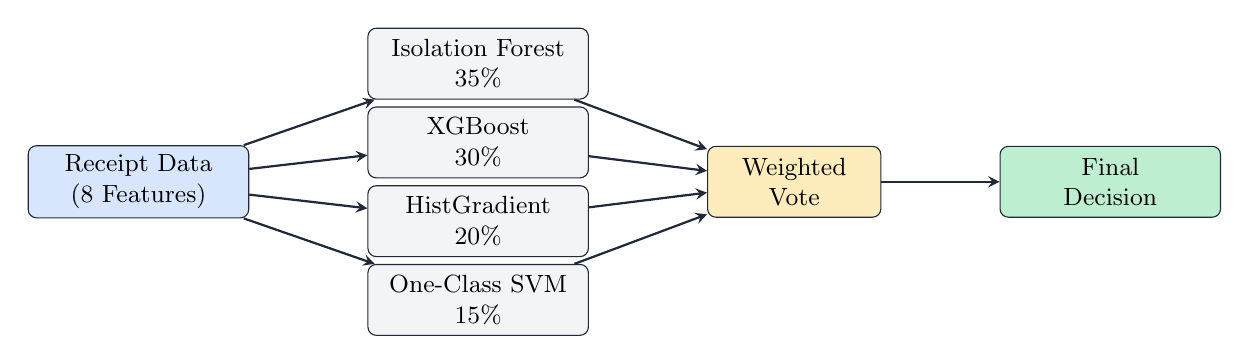
\begin{tikzpicture}[
    node distance=0.8cm,
    box/.style={rectangle, draw=darktext, fill=lightgray, rounded corners=3pt, 
                minimum width=2.8cm, minimum height=0.9cm, align=center, font=\small},
    arrow/.style={->, >=stealth, thick, darktext}
]

% Input
\node[box, fill=primary!20] (input) {Receipt Data\\(8 Features)};

% Models
\node[box, right=1.5cm of input, yshift=1.5cm] (if) {Isolation Forest\\35\%};
\node[box, right=1.5cm of input, yshift=0.5cm] (xgb) {XGBoost\\30\%};
\node[box, right=1.5cm of input, yshift=-0.5cm] (hgb) {HistGradient\\20\%};
\node[box, right=1.5cm of input, yshift=-1.5cm] (svm) {One-Class SVM\\15\%};

% Aggregator
\node[box, right=1.5cm of xgb, yshift=-0.5cm, fill=warning!30, minimum width=2.2cm] (vote) {Weighted\\Vote};

% Output
\node[box, right=1.5cm of vote, fill=success!30] (output) {Final\\Decision};

% Arrows
\draw[arrow] (input) -- (if);
\draw[arrow] (input) -- (xgb);
\draw[arrow] (input) -- (hgb);
\draw[arrow] (input) -- (svm);

\draw[arrow] (if) -- (vote);
\draw[arrow] (xgb) -- (vote);
\draw[arrow] (hgb) -- (vote);
\draw[arrow] (svm) -- (vote);

\draw[arrow] (vote) -- (output);

\end{tikzpicture}
\end{center}

\vspace{2em}

%% ============================================================
%% FIGURE 5: DECISION LOGIC FLOWCHART
%% ============================================================
\section*{Figure 5: Agentic Decision Logic}

\begin{center}
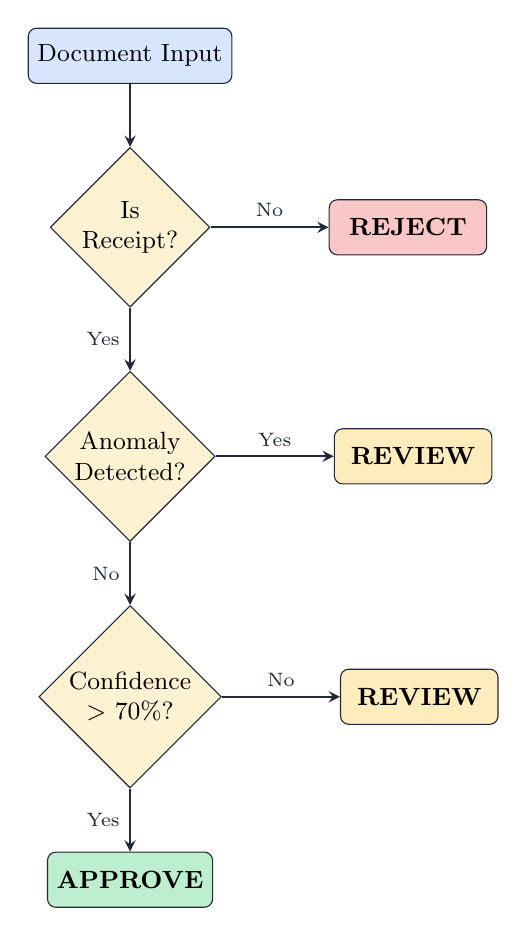
\begin{tikzpicture}[
    node distance=0.6cm,
    decision/.style={diamond, draw=darktext, fill=warning!20, 
                     minimum width=2cm, minimum height=1cm, align=center, font=\small,
                     inner sep=1pt},
    process/.style={rectangle, draw=darktext, fill=lightgray, rounded corners=3pt,
                    minimum width=2.5cm, minimum height=0.7cm, align=center, font=\small},
    outcome/.style={rectangle, draw=darktext, rounded corners=3pt,
                    minimum width=2cm, minimum height=0.7cm, align=center, font=\small\bfseries},
    arrow/.style={->, >=stealth, thick, darktext}
]

% Start
\node[process, fill=primary!20] (start) {Document Input};

% Decision 1
\node[decision, below=0.8cm of start] (d1) {Is\\Receipt?};
\node[outcome, right=1.5cm of d1, fill=danger!30] (reject1) {REJECT};

% Decision 2
\node[decision, below=0.8cm of d1] (d2) {Anomaly\\Detected?};
\node[outcome, right=1.5cm of d2, fill=warning!30] (review1) {REVIEW};

% Decision 3
\node[decision, below=0.8cm of d2] (d3) {Confidence\\$>$ 70\%?};
\node[outcome, right=1.5cm of d3, fill=warning!30] (review2) {REVIEW};

% Final
\node[outcome, below=0.8cm of d3, fill=success!30] (approve) {APPROVE};

% Arrows
\draw[arrow] (start) -- (d1);
\draw[arrow] (d1) -- node[above, font=\scriptsize] {No} (reject1);
\draw[arrow] (d1) -- node[left, font=\scriptsize] {Yes} (d2);
\draw[arrow] (d2) -- node[above, font=\scriptsize] {Yes} (review1);
\draw[arrow] (d2) -- node[left, font=\scriptsize] {No} (d3);
\draw[arrow] (d3) -- node[above, font=\scriptsize] {No} (review2);
\draw[arrow] (d3) -- node[left, font=\scriptsize] {Yes} (approve);

\end{tikzpicture}
\end{center}

\vspace{2em}

%% ============================================================
%% FIGURE 6: THE 4 AGENTS
%% ============================================================
\section*{Figure 6: Agent Architecture}

\begin{center}
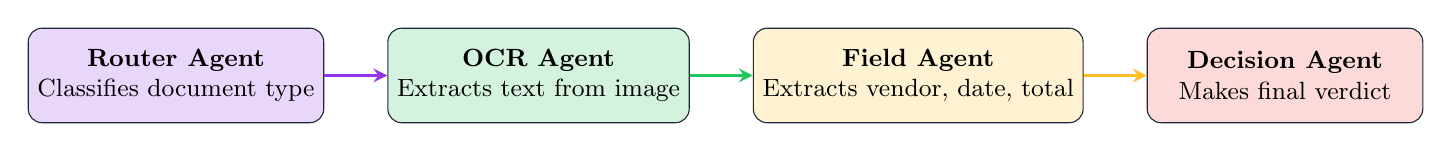
\begin{tikzpicture}[
    node distance=0.3cm,
    agent/.style={rectangle, draw=darktext, rounded corners=5pt,
                  minimum width=3.5cm, minimum height=1.2cm, align=center, font=\small},
    arrow/.style={->, >=stealth, very thick}
]

% Agents
\node[agent, fill=purple!20] (router) {\textbf{Router Agent}\\Classifies document type};
\node[agent, fill=success!20, right=0.8cm of router] (ocr) {\textbf{OCR Agent}\\Extracts text from image};
\node[agent, fill=warning!20, right=0.8cm of ocr] (field) {\textbf{Field Agent}\\Extracts vendor, date, total};
\node[agent, fill=danger!20, right=0.8cm of field] (decision) {\textbf{Decision Agent}\\Makes final verdict};

% Arrows
\draw[arrow, purple] (router) -- (ocr);
\draw[arrow, success] (ocr) -- (field);
\draw[arrow, warning] (field) -- (decision);

\end{tikzpicture}
\end{center}

\vspace{2em}

%% ============================================================
%% FIGURE 7: FEATURE IMPORTANCE BAR CHART
%% ============================================================
\section*{Figure 7: Feature Importance for Auto-Approval}

\begin{center}
\begin{tikzpicture}
    % Y-axis labels and bars
    \def\barheight{0.5}
    \def\gap{0.15}
    \def\scale{0.12}
    
    % Data: feature name, value
    \node[anchor=east, font=\small] at (0, 5*(\barheight+\gap)) {Document Type};
    \fill[primary] (0.1, 5*(\barheight+\gap)-\barheight/2) rectangle (0.1+41*\scale, 5*(\barheight+\gap)+\barheight/2);
    \node[anchor=west, font=\small] at (0.2+41*\scale, 5*(\barheight+\gap)) {41.0\%};
    
    \node[anchor=east, font=\small] at (0, 4*(\barheight+\gap)) {Amount};
    \fill[primary!80] (0.1, 4*(\barheight+\gap)-\barheight/2) rectangle (0.1+14.5*\scale, 4*(\barheight+\gap)+\barheight/2);
    \node[anchor=west, font=\small] at (0.2+14.5*\scale, 4*(\barheight+\gap)) {14.5\%};
    
    \node[anchor=east, font=\small] at (0, 3*(\barheight+\gap)) {Field Completeness};
    \fill[primary!70] (0.1, 3*(\barheight+\gap)-\barheight/2) rectangle (0.1+14*\scale, 3*(\barheight+\gap)+\barheight/2);
    \node[anchor=west, font=\small] at (0.2+14*\scale, 3*(\barheight+\gap)) {14.0\%};
    
    \node[anchor=east, font=\small] at (0, 2*(\barheight+\gap)) {Confidence Score};
    \fill[primary!60] (0.1, 2*(\barheight+\gap)-\barheight/2) rectangle (0.1+12.9*\scale, 2*(\barheight+\gap)+\barheight/2);
    \node[anchor=west, font=\small] at (0.2+12.9*\scale, 2*(\barheight+\gap)) {12.9\%};
    
    \node[anchor=east, font=\small] at (0, 1*(\barheight+\gap)) {Vendor Frequency};
    \fill[primary!50] (0.1, 1*(\barheight+\gap)-\barheight/2) rectangle (0.1+12.8*\scale, 1*(\barheight+\gap)+\barheight/2);
    \node[anchor=west, font=\small] at (0.2+12.8*\scale, 1*(\barheight+\gap)) {12.8\%};
    
    \node[anchor=east, font=\small] at (0, 0*(\barheight+\gap)) {Has Valid Date};
    \fill[primary!40] (0.1, 0*(\barheight+\gap)-\barheight/2) rectangle (0.1+5*\scale, 0*(\barheight+\gap)+\barheight/2);
    \node[anchor=west, font=\small] at (0.2+5*\scale, 0*(\barheight+\gap)) {5.0\%};
    
    % X-axis
    \draw[thick] (0.1, -0.5) -- (6, -0.5);
    \node[font=\small] at (3, -0.9) {Importance Score (\%)};
    
\end{tikzpicture}
\end{center}

\vspace{2em}

%% ============================================================
%% FIGURE 8: ROUTING DISTRIBUTION
%% ============================================================
\section*{Figure 8: Current System Routing Distribution}

\begin{center}
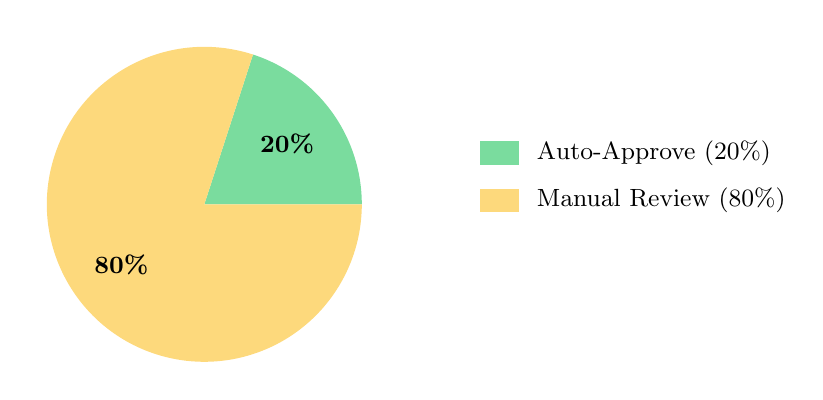
\begin{tikzpicture}
    % Pie chart - manual drawing
    % Auto-approve: 20% = 72 degrees
    % Manual review: 80% = 288 degrees
    
    \fill[success!60] (0,0) -- (0:2) arc (0:72:2) -- cycle;
    \fill[warning!60] (0,0) -- (72:2) arc (72:360:2) -- cycle;
    
    % Labels on pie
    \node[font=\small\bfseries] at (36:1.3) {20\%};
    \node[font=\small\bfseries] at (216:1.3) {80\%};
    
    % Legend
    \fill[success!60] (3.5, 0.5) rectangle (4, 0.8);
    \node[anchor=west, font=\small] at (4.1, 0.65) {Auto-Approve (20\%)};
    
    \fill[warning!60] (3.5, -0.1) rectangle (4, 0.2);
    \node[anchor=west, font=\small] at (4.1, 0.05) {Manual Review (80\%)};
    
\end{tikzpicture}
\end{center}

\begin{center}
\textit{Conservative by design: prioritizing accuracy over automation}
\end{center}

\vspace{2em}

%% ============================================================
%% FIGURE 9: COMBINED RESULTS TABLE
%% ============================================================
\section*{Figure 9: Combined System Results}

\begin{table}[H]
\centering
\renewcommand{\arraystretch}{1.4}
\begin{tabular}{l c c}
\toprule
\rowcolor{lightgray}
\textbf{Component} & \textbf{Metric} & \textbf{Result} \\
\midrule
Document Classification & Accuracy & 98.0\% \\
\rowcolor{lightgray!30}
LayoutLM Field Extraction & Accuracy & 99.08\% \\
OCR Processing & Avg. Confidence & 75\%+ \\
\rowcolor{lightgray!30}
Anomaly Detection (Ensemble) & Accuracy & 98.0\% \\
Ensemble Improvement & vs. Best Individual & +9.1\% \\
\bottomrule
\end{tabular}
\caption*{\textbf{End-to-End Pipeline Performance}}
\end{table}

\vspace{2em}

%% ============================================================
%% FIGURE 10: PROCESSING SPEED
%% ============================================================
\section*{Figure 10: Processing Speed Breakdown}

\begin{center}
\begin{tikzpicture}
    % Horizontal bar chart for timing
    \def\barheight{0.6}
    \def\gap{0.3}
    \def\scale{0.008}
    
    \node[anchor=east, font=\small] at (0, 3*(\barheight+\gap)) {OCR Processing};
    \fill[danger!60] (0.1, 3*(\barheight+\gap)-\barheight/2) rectangle (0.1+450*\scale, 3*(\barheight+\gap)+\barheight/2);
    \node[anchor=west, font=\small] at (0.2+450*\scale, 3*(\barheight+\gap)) {450ms};
    
    \node[anchor=east, font=\small] at (0, 2*(\barheight+\gap)) {Field Extraction};
    \fill[warning!60] (0.1, 2*(\barheight+\gap)-\barheight/2) rectangle (0.1+100*\scale, 2*(\barheight+\gap)+\barheight/2);
    \node[anchor=west, font=\small] at (0.2+100*\scale, 2*(\barheight+\gap)) {100ms};
    
    \node[anchor=east, font=\small] at (0, 1*(\barheight+\gap)) {Classification};
    \fill[primary!60] (0.1, 1*(\barheight+\gap)-\barheight/2) rectangle (0.1+25*\scale, 1*(\barheight+\gap)+\barheight/2);
    \node[anchor=west, font=\small] at (0.2+25*\scale, 1*(\barheight+\gap)) {25ms};
    
    \node[anchor=east, font=\small] at (0, 0*(\barheight+\gap)) {Anomaly Detection};
    \fill[success!60] (0.1, 0*(\barheight+\gap)-\barheight/2) rectangle (0.1+25*\scale, 0*(\barheight+\gap)+\barheight/2);
    \node[anchor=west, font=\small] at (0.2+25*\scale, 0*(\barheight+\gap)) {25ms};
    
    % Total
    \draw[thick, dashed] (0.1, -0.7) -- (5.5, -0.7);
    \node[font=\small\bfseries] at (2.5, -1.1) {Total: $\sim$600ms per receipt};
    
\end{tikzpicture}
\end{center}

\vspace{2em}

%% ============================================================
%% FIGURE 11: KEY TAKEAWAYS
%% ============================================================
\section*{Figure 11: Key Takeaways}

\begin{tcolorbox}[colback=lightgray, colframe=darktext, arc=3mm, boxrule=0.5pt]
\begin{enumerate}[leftmargin=*, itemsep=0.5em]
    \item \textbf{Ensembles Work} --- 9\% improvement over best individual model
    \item \textbf{Explainability Matters} --- System explains WHY something is flagged
    \item \textbf{Agents $>$ Pipelines} --- Retry logic and fallbacks for robustness
    \item \textbf{Feedback Loop} --- Gets smarter without manual retraining
    \item \textbf{Conservative Design} --- Accuracy prioritized over automation
\end{enumerate}
\end{tcolorbox}

\vspace{2em}

%% ============================================================
%% FIGURE 12: ANOMALY EXPLANATION EXAMPLE
%% ============================================================
\section*{Figure 12: Explainable Anomaly Output}

\begin{tcolorbox}[colback=danger!10, colframe=danger, arc=3mm, boxrule=1pt, title={\textbf{Anomaly Detected}}]
\textbf{Prediction:} ANOMALY \\
\textbf{Confidence:} 82\%

\vspace{0.5em}
\textbf{Reasons:}
\begin{itemize}[leftmargin=*, itemsep=0.2em]
    \item High amount: \$50,000.00
    \item Missing or invalid vendor
    \item Invalid or missing date
\end{itemize}

\vspace{0.5em}
\textbf{Action:} Flagged for human review
\end{tcolorbox}

\vspace{2em}

%% ============================================================
%% FIGURE 13: HUMAN-IN-THE-LOOP DIAGRAM
%% ============================================================
\section*{Figure 13: Human-in-the-Loop Feedback}

\begin{center}
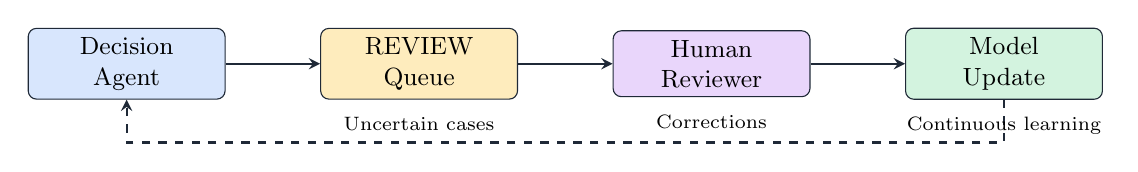
\begin{tikzpicture}[
    node distance=0.5cm,
    box/.style={rectangle, draw=darktext, rounded corners=3pt, 
                minimum width=2.5cm, minimum height=0.8cm, align=center, font=\small},
    arrow/.style={->, >=stealth, thick, darktext}
]

% Flow
\node[box, fill=primary!20] (agent) {Decision\\Agent};
\node[box, fill=warning!30, right=1.2cm of agent] (review) {REVIEW\\Queue};
\node[box, fill=purple!20, right=1.2cm of review] (human) {Human\\Reviewer};
\node[box, fill=success!20, right=1.2cm of human] (update) {Model\\Update};

% Arrows
\draw[arrow] (agent) -- (review);
\draw[arrow] (review) -- (human);
\draw[arrow] (human) -- (update);

% Feedback loop
\draw[arrow, dashed] (update) -- ++(0, -1) -| (agent);

% Labels
\node[font=\scriptsize, below=0.1cm of review] {Uncertain cases};
\node[font=\scriptsize, below=0.1cm of human] {Corrections};
\node[font=\scriptsize, below=0.1cm of update] {Continuous learning};

\end{tikzpicture}
\end{center}

\vspace{2em}

%% ============================================================
%% FIGURE 14: WHAT ANOMALY DETECTION CATCHES
%% ============================================================
\section*{Figure 14: What Anomaly Detection Catches}

\begin{table}[H]
\centering
\renewcommand{\arraystretch}{1.3}
\begin{tabular}{l l}
\toprule
\rowcolor{lightgray}
\textbf{Anomaly Type} & \textbf{Example} \\
\midrule
Unusually high amounts & \$50,000 for coffee \\
\rowcolor{lightgray!30}
Missing critical fields & No vendor name \\
Invalid dates & February 30th, 2025 \\
\rowcolor{lightgray!30}
Suspicious timing & 3 AM transactions \\
Data integrity issues & Negative totals \\
\rowcolor{lightgray!30}
Statistical outliers & 500 items on one receipt \\
\bottomrule
\end{tabular}
\caption*{\textbf{Types of Anomalies Detected}}
\end{table}

\vspace{3em}

\begin{center}
\rule{0.8\textwidth}{0.5pt}\\[1em]
{\small\textit{End of figures. Compile with pdflatex and screenshot as needed.}}
\end{center}

\end{document}




